\documentclass{beamer}

\usetheme{Montpellier}
%\usetheme{CambridgeUS}


\usepackage[OT1]{fontenc}
\usepackage[utf8x]{inputenc}


%\usepackage[T1]{fontenc}
%\usepackage[latin9]{inputenc}
\usepackage[german]{babel}
\usepackage{booktabs,bm, color, enumerate, hyperref, pgf, url, soul, tikz}
\usepackage{amssymb, amsmath}
\usepackage{graphicx}
\newcommand*{\Scale}[2][4]{\scalebox{#1}{$#2$}}%
\newcommand*{\Resize}[2]{\resizebox{#1}{!}{$#2$}}%
\usepackage{listings}
\usepackage{adjustbox}
%\usepackage{hyperref}

\usepackage{appendixnumberbeamer}


\bibliographystyle{apalike}



%\input{abbreviations}



\setbeamertemplate{blocks}[rounded][shadow=true]
%\usepackage{appendixnumberbeamer}



%\subject{2015}




\title{Advanced Regression: 2c Distributed non-linear lag models and other extensions}



\author{Garyfallos Konstantinoudis}
\institute{Epidemiology and Biostatistics, Imperial College London}



\date{28th February 2023}

\setlength{\unitlength}{0.9cm}
\linethickness{1.1pt}


\begin{document}

\frame{
	\titlepage
}



\frame{
	\tableofcontents
}


\frame{
	\frametitle{Overview} 
	
	Concepts we cover in this lecture:
	\begin{itemize}
		\item Distributed lag non-linear models
		\item Cross-basis function
		\item Case studies
	\end{itemize}
	
	
}

\section{Introduction to lags}
\frame{
	\frametitle{Introduction of the problem} 
	
	\begin{itemize}
		\item An exposure event is frequently associated with a risk lasting for a defined period in the future
		\item The risk at a given time is assumed a result of protracted exposures experienced in the past

		\item Examples include, drugs, carcinogens, etc. 
	\end{itemize}
	
	Challenge: The risk should be modelled in terms of contributions depending on
	intensity and timing of the exposure events: bi-dimensional association
(interaction)
}

\section{Example 1: Lung cancer and radon exposure}

\frame{
	\frametitle{Example 1: Lung cancer and radon exposure} 
	
	\begin{figure}
	\centering	
	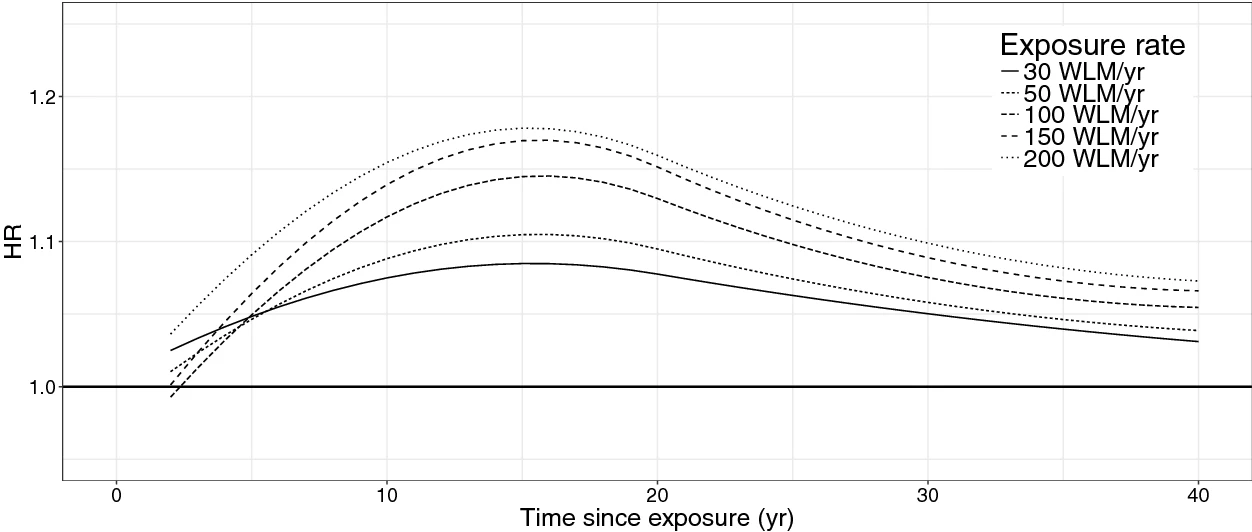
\includegraphics[width = 10cm]{E:/Postdoc Imperial/Lectures/2023_AdvancedRegression/AdvancedRegression2022-2023/lectures/graphs/radonlung.png}	
\end{figure}
}

\section{Example 2: PM10 in Chicago}

\begin{frame}[fragile]{Example 2: PM10 in Chicago}
	\begin{lstlisting}[language=R, basicstyle=\tiny]
k <- 1:16
res_store <- list()

for(i in 1:length(k)){
chicagoNMMAPS$pm10_laggeg <- lag(chicagoNMMAPS$pm10, n = k[i]-1)

mgcv::gam(death ~ s(temp) + 
	s(time) + s(month) + dow + pm10_laggeg, 
	data = chicagoNMMAPS, family = "poisson") -> tmp

res_store[[i]] <- list(est = coef(tmp)["pm10_laggeg"] , 
	LL = coef(tmp)["pm10_laggeg"] - 1.96*summary(tmp)$se["pm10_laggeg"],
	UL = coef(tmp)["pm10_laggeg"] + 1.96*summary(tmp)$se["pm10_laggeg"])
}

lapply(res_store, unlist) %>% do.call(rbind, .) %>% as_tibble() %>% mutate(type = 
	factor(paste0("lag ", 0:15), levels = paste0("lag ", 0:15))) -> plotres

ggplot(data = plotres) + 
	geom_point(aes(x=type, y=est.pm10_laggeg)) + 
	geom_errorbar(aes(x=type, ymin=LL.pm10_laggeg, ymax=UL.pm10_laggeg, width = 0.1)) + 
	geom_hline(yintercept = 0, col = "red", linetype = "dotted") + theme_bw() +
	ylab("log risk PM10") + xlab("Lags") |

ggplot(data = plotres) + 
	geom_point(aes(x=type, y=est.pm10_laggeg)) + 
	geom_line(aes(x=type, y=est.pm10_laggeg, group=1)) +
	geom_ribbon(aes(x=type, ymin=LL.pm10_laggeg, ymax=UL.pm10_laggeg, group = 1), 
	fill = "blue", alpha = 0.2) + geom_hline(yintercept = 0, col = "red", 
	linetype = "dotted") + theme_bw() + ylab("log risk PM10") + xlab("Lags") 
	\end{lstlisting}
	
\end{frame}

\frame{
	\frametitle{Example 2: PM10 in Chicago} 
	\begin{itemize}
		\item Which are the main assumptions here?
	\end{itemize}
	\begin{figure}
		\centering	
		\includegraphics[width = 9cm]{E:/Postdoc Imperial/Lectures/2023_AdvancedRegression/AdvancedRegression2022-2023/lectures/graphs/p29.png}	
	\end{figure}
}


\section{Distributed linear lag models}

\frame{
	\frametitle{Distributed linear lag models} 
	The unconstrained distributed lag model of order q is:
	$$Y_t = \beta_0 + \beta_{10}X_t + \beta_{11}X_{t-1} + \dots+ \beta_{1q}X_{t-q} + \epsilon_t$$
	\begin{itemize}
		\item $\beta_{1\ell}$ is the effect at lag $\ell=0, 1, \dots q$ and $\epsilon_t$ an error term.
		\item The \textcolor{red}{overall impact} for a unit change in $X$ is given by $\sum^q_{\ell=0}\beta_\ell$.
	\end{itemize}
}


\begin{frame}[fragile]{Example 2: PM10 in Chicago}
	\begin{lstlisting}[language=R, basicstyle=\tiny]
chicagoNMMAPS$pm10_laggeg0 <- lag(chicagoNMMAPS$pm10, n = 0)
chicagoNMMAPS$pm10_laggeg1 <- lag(chicagoNMMAPS$pm10, n = 1)
chicagoNMMAPS$pm10_laggeg2 <- lag(chicagoNMMAPS$pm10, n = 2)
chicagoNMMAPS$pm10_laggeg3 <- lag(chicagoNMMAPS$pm10, n = 3)

mgcv::gam(death ~ s(temp) + 
	s(time) + s(month) + dow + pm10_laggeg0 + pm10_laggeg1 + pm10_laggeg2 +
	pm10_laggeg3, data = chicagoNMMAPS, family = "poisson") %>% summary()
	
Formula:
death ~ s(temp) + s(time) + s(month) + dow + pm10_laggeg0 + pm10_laggeg1 + 
pm10_laggeg2 + pm10_laggeg3

Parametric coefficients:
Estimate Std. Error z value Pr(>|z|)    
(Intercept)   4.707e+00  5.825e-03 808.083  < 2e-16 ***
dowMonday     2.898e-02  5.375e-03   5.391 7.01e-08 ***
dowTuesday    2.326e-02  5.428e-03   4.285 1.82e-05 ***
dowWednesday  5.054e-03  5.447e-03   0.928 0.353471    
dowThursday   5.898e-03  5.385e-03   1.095 0.273448    
dowFriday     1.294e-02  5.336e-03   2.426 0.015264 *  
dowSaturday   1.931e-02  5.273e-03   3.661 0.000251 ***
pm10_laggeg0  3.958e-04  8.997e-05   4.399 1.09e-05 ***
pm10_laggeg1  1.765e-04  9.259e-05   1.907 0.056571 .  
pm10_laggeg2 -2.595e-05  9.039e-05  -0.287 0.774093    
pm10_laggeg3  1.188e-04  8.350e-05   1.423 0.154769   
	\end{lstlisting}
\end{frame}

\frame{
	\frametitle{Considerations} 
	\begin{itemize}
		\item Easy implementation when lags are few; overparametrized when we want to assess a lot of lags
		\item Collinearity issues: The exposure is likely to be highly correlated with the values of the previous/after days. Weird behaviours in the point estimates (surprising protective effects), variance inflation. 
	\end{itemize}
Alternative: to impose some constraints:
	\begin{itemize}
	\item A constant effect within lag intervals
	\item Average of the exposures in the previous $L$ day 
	\item Describing the coefficients with a smooth curve using continuous functions such as splines, polynomials, and other basis functions.
\end{itemize}
The idea: $\beta_{\ell}$ can be modelled using a basis function. 
}



\frame{
	\frametitle{Polynomial DLM} 
	
	Let $\beta_\ell = \sum_j^p\tau_j\ell^j, \;\;\; \ell = 0, \dots, q$, lets write it for 2 lags using a 3rd degree polynomial to see it explicitly: 
	\begin{align*}
	Y_t &= \beta_0 + \beta_{10}X_t + \beta_{11}X_{t-1} + \beta_{12}X_{t-2} + \epsilon_t\\
	\beta_{10} &= \tau_0, \; \beta_{11} = \tau_0 + \tau_1 + \tau_2 + \tau_3, \; \beta_{12} = \tau_0 + \tau_1 2  + \tau_2 2^2 + \tau_3 2^3
	\end{align*}
		and we can modify as per first lecture to model more localized structures using: $\beta_\ell = \sum_j^p\tau_j\ell^j + \sum_k^K\nu_k(\ell-\kappa_k)^p_+$, thus:
		\begin{align*}
	\beta_{10} &= \tau_0 + \nu_1(0-\kappa_1)^3_+ + \dots + \nu_K(0-\kappa_K)^3_+, \\
	\beta_{11} &= \tau_0 + \tau_1 + \tau_2 + \tau_3 + \nu_1(1-\kappa_1)^3_+ + \dots + \nu_K(1-\kappa_K)^3_+, \\
	\beta_{12} &= \tau_0 + \tau_1 2  + \tau_2 2^2 + \tau_3 2^3 + \nu_1(2-\kappa_1)^3_+ + \dots + \nu_K(2-\kappa_K)^3_+
	\end{align*}
	
	and similarly we can penalize it can estimate the \textit{penalised spline distributed lag estimate} of $\beta_{\ell}$
}


\begin{frame}[fragile]{Polynomial DLM in R: Chicago}
	\begin{lstlisting}[language=R, basicstyle=\tiny]
cb1.pm <- crossbasis(chicagoNMMAPS$pm10, lag=15, argvar=list(fun="lin"),
	arglag=list(fun="poly", degree=4))
	
summary(cb1.pm)

CROSSBASIS FUNCTIONS
observations: 5114 
range: -3.049835 to 356.1768 
lag period: 0 15 
total df:  5 

BASIS FOR VAR:
fun: lin 
intercept: FALSE 

BASIS FOR LAG:
fun: poly 
degree: 4 
scale: 15 
intercept: TRUE 

model_dlm <- mgcv::gam(death ~ s(temp) + s(time) + s(month) + dow + cb1.pm,
	family=poisson(), chicagoNMMAPS)
	
summary(model_dlm)

pred1.pm <- crosspred(cb1.pm, model_dlm, at=0:20, bylag=0.2)
plot(pred1.pm, ptype = "slices", var = 1, cumul=FALSE, ylab="RR",
	 main="Association with a 1-unit increase in PM10")
	\end{lstlisting}
\end{frame}

\begin{frame}[fragile]{Polynomial DLM in R: Chicago}
	\begin{lstlisting}[language=R, basicstyle=\tiny]
Family: poisson 
Link function: log 

Formula:
death ~ s(temp) + s(time) + s(month) + dow + cb1.pm

Parametric coefficients:
Estimate Std. Error z value Pr(>|z|)    
(Intercept)   4.734e+00  1.028e-02 460.746  < 2e-16 ***
dowMonday     3.162e-02  5.933e-03   5.330 9.85e-08 ***
dowTuesday    2.100e-02  5.998e-03   3.501 0.000463 ***
dowWednesday  3.579e-03  6.050e-03   0.592 0.554073    
dowThursday   3.367e-03  6.069e-03   0.555 0.579092    
dowFriday     1.339e-02  6.054e-03   2.212 0.026984 *  
dowSaturday   1.805e-02  5.957e-03   3.031 0.002439 ** 
cb1.pmv1.l1   3.062e-04  7.862e-05   3.895 9.81e-05 ***
cb1.pmv1.l2  -2.115e-03  1.068e-03  -1.979 0.047789 *  
cb1.pmv1.l3   3.966e-03  4.423e-03   0.897 0.369884    
cb1.pmv1.l4  -3.477e-03  6.698e-03  -0.519 0.603653    
cb1.pmv1.l5   1.348e-03  3.323e-03   0.406 0.684882    

Approximate significance of smooth terms:
edf Ref.df Chi.sq p-value    
s(temp)  8.584  8.940  165.0  <2e-16 ***
s(time)  7.658  8.530  261.1  <2e-16 ***
s(month) 8.125  8.806  278.3  <2e-16 ***

R-sq.(adj) =  0.267   Deviance explained = 29.1%
	\end{lstlisting}
\end{frame}

\begin{frame}[fragile]{Polynomial DLM in R: Chicago}
	\begin{itemize}
		\item Retrieve the cumulative effect. What is the interpretation here?
	\end{itemize}
	\begin{lstlisting}[language=R, basicstyle=\tiny]
> pred1.pm$allRRfit["1"]
1 
0.9997201 
> pred1.pm$allRRlow["1"]
1 
0.9991616 
> pred1.pm$allRRhigh["1"]
1 
1.000279 
	\end{lstlisting}
\end{frame}


\begin{frame}[fragile]{Polynomial DLM in R: Chicago}
What is the main assumption here? Can we relax it?
	\begin{figure}
	\centering	
	\includegraphics[width = 9cm]{E:/Postdoc Imperial/Lectures/2023_AdvancedRegression/AdvancedRegression2022-2023/lectures/graphs/p30.png}	
\end{figure}
\end{frame}

\section{Distributed non-linear lag models}

\begin{frame}[fragile]{Extension to distributed non-linear lag models}
	\begin{itemize}
		\item We know that temperature and mortality have a U-shape relationship
		\item We know that high temperature has a lag effect on mortality
		\item Can we define models to combine these two components?
	\end{itemize}

The idea: to calculate this bi-dimensional relationship, we need a basis function that combines the basis function in the lag dimension and the basis function in the exposure dimension: \textbf{Cross-basis function}
	
\end{frame}


\begin{frame}[fragile]{linear-by-constant}
	\begin{figure}
	\centering	
	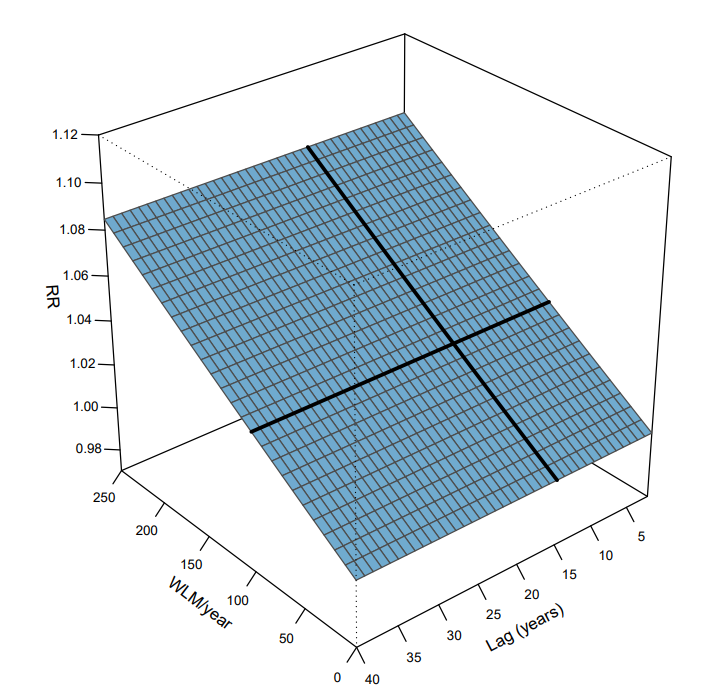
\includegraphics[width = 7cm]{E:/Postdoc Imperial/Lectures/2023_AdvancedRegression/AdvancedRegression2022-2023/lectures/graphs/dlnm1.png}	
\end{figure}
\end{frame}

\begin{frame}[fragile]{spline-by-constant}
	\begin{figure}
		\centering	
		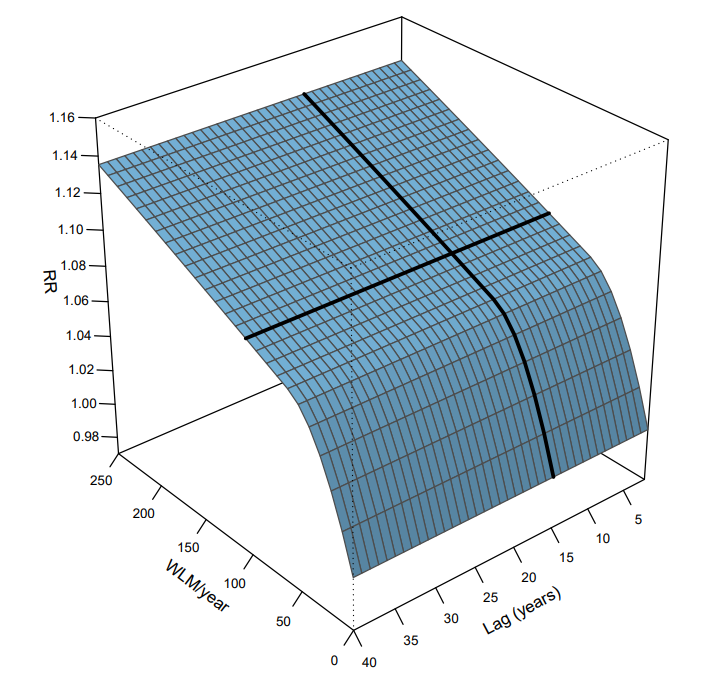
\includegraphics[width = 7cm]{E:/Postdoc Imperial/Lectures/2023_AdvancedRegression/AdvancedRegression2022-2023/lectures/graphs/dlnm2.png}	
	\end{figure}
\end{frame}

\begin{frame}[fragile]{step-by-step}
	\begin{figure}
		\centering	
		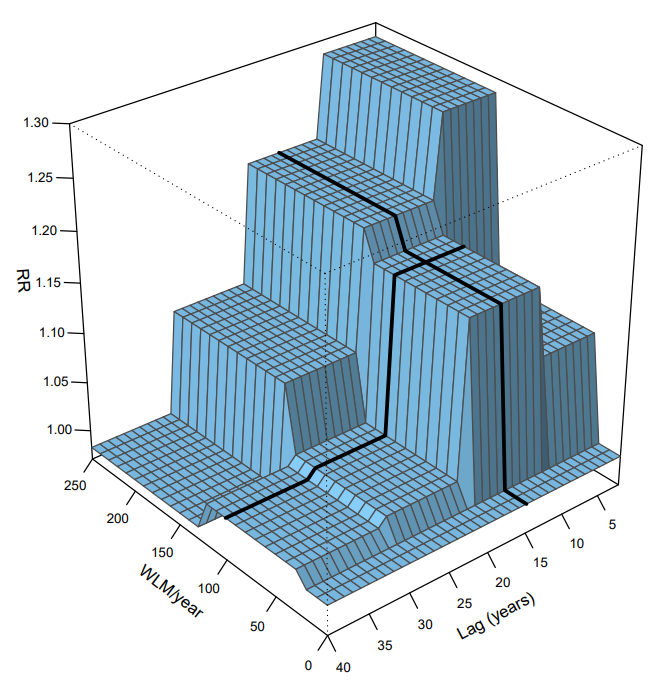
\includegraphics[width = 7cm]{E:/Postdoc Imperial/Lectures/2023_AdvancedRegression/AdvancedRegression2022-2023/lectures/graphs/dlnm3.png}	
	\end{figure}
\end{frame}

\begin{frame}[fragile]{spline-by-spline}
	\begin{figure}
		\centering	
		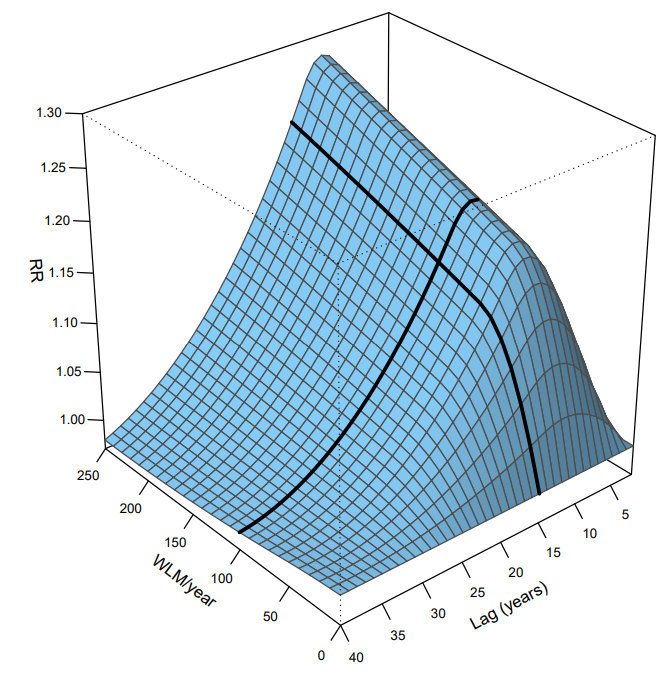
\includegraphics[width = 7cm]{E:/Postdoc Imperial/Lectures/2023_AdvancedRegression/AdvancedRegression2022-2023/lectures/graphs/dlnm4.png}	
	\end{figure}
\end{frame}

\section{Example 3: Temperature in Chicago}

\begin{frame}[fragile]{Example 3: Temperature in Chicago}
	\begin{lstlisting}[language=R, basicstyle=\tiny]
cb2.pm <- crossbasis(chicagoNMMAPS$pm10, lag=1, argvar=list(fun="lin"),
	arglag=list(fun="strata"))

varknots <- equalknots(chicagoNMMAPS$temp, fun="bs", df=5, degree=2)
lagknots <- logknots(10, 3)
cb2.temp <- crossbasis(chicagoNMMAPS$temp, lag=10, argvar=list(fun="bs",
	knots=varknots), arglag=list(knots=lagknots))


model_dlm2 <- mgcv::gam(death ~ cb2.pm + cb2.temp + s(time) + s(month) + dow,
	family=poisson(), chicagoNMMAPS)

pred2.temp <- crosspred(cb2.temp, model_dlm2, cen=21, by=1)

plot(pred2.temp, xlab="Temperature", zlab="RR", theta=200, phi=40, lphi=100,
	main="3D graph of temperature effect")

plot(pred2.temp, "contour", xlab="Temperature", key.title=title("RR"),
plot.title=title("Contour plot",xlab="Temperature",ylab="Lag"))
	\end{lstlisting}
\end{frame}


\begin{frame}{Example 3: Temperature in Chicago}
\begin{columns}
	\column{.5\textwidth}
	\includegraphics[width = 6cm]{E:/Postdoc Imperial/Lectures/2023_AdvancedRegression/AdvancedRegression2022-2023/lectures/graphs/p31.png}
	\column{.5\textwidth}
	\includegraphics[width = 6cm]{E:/Postdoc Imperial/Lectures/2023_AdvancedRegression/AdvancedRegression2022-2023/lectures/graphs/p32.png}
\end{columns}
\end{frame}



\begin{frame}[fragile]{Example 3: Temperature in Chicago}
		\begin{lstlisting}[language=R, basicstyle=\tiny]
plot(pred2.temp, "slices", var=30, col=1, ylim=c(0.95,1.2), lwd=1.5,
main="Lag-response curves for different temperatures, ref. 21C")
	\end{lstlisting}
		\begin{figure}
		\includegraphics[width = 7cm]{E:/Postdoc Imperial/Lectures/2023_AdvancedRegression/AdvancedRegression2022-2023/lectures/graphs/p33.png}	
	\end{figure}
\end{frame}

\begin{frame}[fragile]{Example 3: Temperature in Chicago}
\begin{lstlisting}[language=R, basicstyle=\tiny]
plot(pred2.temp, "slices", var=c(-20,33), lag=c(0,5), col=4,
ci.arg=list(density=40,col=grey(0.7)))
\end{lstlisting}	
		\begin{figure}
	\includegraphics[width = 8cm]{E:/Postdoc Imperial/Lectures/2023_AdvancedRegression/AdvancedRegression2022-2023/lectures/graphs/p34.png}	
\end{figure}
\end{frame}

\section{Example 4: Extension to space}

\begin{frame}[fragile]{Example 4: Extension to space}
Warm temperatures and COPD hospitalisations in England: A nationwide case-crossover study during 2007-2018.
    \begin{columns}
	\column{.5\textwidth}
	\begin{itemize}
		\item 3$^{\text{rd}}$ cause of death, 3.17 million deaths in 2015 globally.
		\item In England, 115,000 emergency admissions and 24,000 deaths per year.
		\item COPD exacerbations: Bacteria, viruses and air-pollution.
		\item The role of temperature is unclear. 
	\end{itemize}
	\column{.5\textwidth}
	\includegraphics[width = 6cm]{E:/Postdoc Imperial/Lectures/2023_AdvancedRegression/AdvancedRegression2022-2023/lectures/graphs/COPD_HES.jpg}
\end{columns}
\end{frame}


%------------- 
\begin{frame}{Temperature}
	\begin{columns}
		\column{.5\textwidth}
		\begin{itemize}
			\item Typically U-shaped relationship between temperature and health.
			\item Cold, dry air or hot air can trigger a flare-up.
			\item Different confounding, different lags across different temperatures.
			\item This study focuses on warm temperatures.
		\end{itemize}
		\column{.5\textwidth}
		\includegraphics[width = 6cm]{E:/Postdoc Imperial/Lectures/2023_AdvancedRegression/AdvancedRegression2022-2023/lectures/graphs/TemperatureHealth.PNG}
	\end{columns}
	
	% add here the histogram
\end{frame}
%------------- 

\begin{frame}{Previous studies}
	
	\vspace{-0.5cm}
	\begin{table}[]
		\begin{adjustbox}{width=\columnwidth,center}
			\begin{tabular}{ccccc}
				\hline
				\hline
				\textbf{Authors} & \textbf{Aggregation} & \textbf{Country} & \textbf{Pollutants} & \textbf{Effect}\\ \hline
				\hline
				Michelozzi 2009 et al & city \& daily & EU & $\text{NO}_{2}$, $\text{O}_{3}$ & 2.1 (0.6 to 3.6) per 1$^o$C \\
				Anderson et al 2013 & county \& daily & US & $\text{O}_{3}$, $\text{PM}_{10}$, $\text{PM}_{2.5}$ & 2.0 (0.4, 4.5) per 10$^o$F \\
				Zhao 2019 et al  & individual & Brazil & no adjustment & 5.0 (4.0, 6.0) per 5$^o$C \\
				\hline
				\hline
			\end{tabular}
		\end{adjustbox}
	\end{table}
	\begin{itemize}
		\item Spatial \& temporal aggregation
		\begin{itemize}
			\item Exposure varies on high resolution.
			\item Insufficient adjustment for confounding (for instance physical activity).
			\item Ecological bias
		\end{itemize}
		\item One study individual data, but did not adjust for air-pollution
	\end{itemize}
\end{frame}



%------------- 
\begin{frame}{Outcome and Exposure}
	\begin{columns}
		\column{0.55\textwidth}
		Outcome
		\begin{itemize}
			\item NHS digital \& SAHSU. 
			\item COPD hospitalization (ICD10 J40-44) 2007-2018.
			\item Individual data/ 100m grid spatial resolution.
			\item Summer months.
		\end{itemize}
		Exposure
		\begin{itemize}
			\item Daily maximum temperature 2007-2018 at 1km grid from MetOffice.
			\item lag0-2.
		\end{itemize}
		\column{0.45\textwidth}
		\includegraphics[width=50mm,scale=1]{E:/Postdoc Imperial/Lectures/2023_AdvancedRegression/AdvancedRegression2022-2023/lectures/graphs/temperatureLTLA.png}
	\end{columns}
\end{frame}
%------------- 

%------------- Confounding
\begin{frame}{Confounding}
	\vspace{-1cm}
	\begin{figure}
		\centering
		\includegraphics[width=8cm]{E:/Postdoc Imperial/Lectures/2023_AdvancedRegression/AdvancedRegression2022-2023/lectures/graphs/copdDAG.pdf}
	\end{figure}
	
\end{frame}
%------------- 

%------------- Confounding
\begin{frame}{Covariates}
	\vspace{-0.5cm}
	\centering
	{\fontsize{9}{10}\selectfont
		\begin{table}[!t]
			\begin{tabular}{lcccc}
				\hline
				Covariates & Source & Space & Time & years \\ \hline
				PM$_{2.5}$ & \href{https://catalogue.ceda.ac.uk/uuid/4dc8450d889a491ebb20e724debe2dfb
				}{MetOffice} & 1km$^2$ & daily & 2007-2018\\
				O$_{3}$ & \href{https://catalogue.ceda.ac.uk/uuid/4dc8450d889a491ebb20e724debe2dfb
				}{MetOffice} & 1km$^2$ & daily & 2007-2018\\
				Relative humidity & \href{https://catalogue.ceda.ac.uk/uuid/4dc8450d889a491ebb20e724debe2dfb
				}{MetOffice} & 10km$^2$ & daily & 2007-2018\\
				Holidays & ONS & nationwide & daily & 2007-2018\\
				\hline
			\end{tabular}
		\end{table}
	}
	
\end{frame}
%------------- 

%------------- Spatial effect modifiers 
\begin{frame}{Spatial effect modifiers }
	\vspace{-0.5cm}
	\hspace{-0.7cm}
	\includegraphics[width=11.5cm]{E:/Postdoc Imperial/Lectures/2023_AdvancedRegression/AdvancedRegression2022-2023/lectures/graphs/SpatEffMod.png}
\end{frame}
%------------- 


%------------- 
\begin{frame}{Step 1. Find linear threshold}
	
	Let $Y_{ij}$ be  an indicator of the COPD hospitalization at time i (1-case, 0-control) of the j-th group of cases-controls, and $\mu_{ij}$ the risk ratio: \vspace{-0.5cm}
	\begin{align*}
	Y_{ij}  &\sim \text{Poisson}(\mu_{ij}) \nonumber\\
	\log(\mu_{ijk})  & = \alpha_1 I(X_{1i}< c_l) X_{1i} + \alpha_2 I(X_{1i}\geq c_l)X_{1i} + \\ &  \quad\quad \sum_{m=1}^4\beta_mZ_{mi} + u_{j} + w_k \nonumber\\
	u_j & \sim N(0, 100)\nonumber\\
	w_k & \sim N(0, \sigma^2)\nonumber\\
	\alpha_1, \alpha_2, \beta_1, \dots \beta_4 & \sim N(0, 1)\nonumber\\
	\sigma & \sim \text{Gamma}(p, q) \nonumber
	\end{align*} 
\end{frame}
%------------- 

%------------- 
\begin{frame}{Step 2a. Effect modification by age and sex}
	
	We fitted the previous model for $c_*$ that minimizes the WAIC for the different sex and age group ($<$65, 65$-$85, $>$85) $g$ subgroups and patient $k$.
	\begin{align*}
	Y_{ijgk} & \sim \text{Poisson}(\mu_{ijgk}) \nonumber\\
	\log(\mu_{ijgk}) & = \alpha_1 I(X_{1ig}< c_*) X_{1ig} + \alpha_2 I(X_{1ig}\geq c_*)X_{1igk} + \\ &  \quad\quad \sum_{m=1}^4\beta_mZ_{mig} + u_{j} + w_k\nonumber\\
	u_j &\sim N(0, 100)\nonumber\\
	w_k & \sim N(0, \sigma^2)\nonumber\\
	\alpha_1, \alpha_2, \beta_1, \dots \beta_5 &\sim N(0, 1)\nonumber\\
	\end{align*} 
	
\end{frame}
%------------- 

%------------- 
\begin{frame}{Step 2b. Spatial Effect modification}
	\vspace{-1cm}
	{\small
		\begin{columns}
			\column{0.40\textwidth}
			\begin{align*}
			Y_{ijk} & \sim \text{Poisson}(\mu_{ijk}) \nonumber\\
			\log(\mu_{ijk}) & = \alpha_1 I(X_{1i}< c_*)X_{1i} + \alpha_{2s} I(X_{1i}\geq c_*)X_{1i} + \\ &  \quad\quad \sum_{m=1}^4\beta_mZ_{mi} + u_{j} + w_k\nonumber\\
			\alpha_{2s} &= \alpha_2 + \sum_{m=1}^8 \gamma_m H_{sm} + v_s + b_s \nonumber\\
			w_k & \sim N(0, \sigma_1^2)\nonumber\\
			v_s &\sim N(0, \sigma_2^2)\nonumber\\
			b_s|b_{-s} &\sim N\bigg(\frac{\sum_{s \sim r} w_{rs} b_s}{\sum_{s \sim r} w_{rs}},        \frac{\sigma^3_2}{\sum_{s \sim r} w_{rs}}\bigg) \nonumber\\
			% u_j &\sim N(0, 100)\nonumber\\
			% \alpha_1, \alpha_2, \beta_1, \dots \beta_4, \gamma_1, \dots, \gamma_8 &\sim N(0,        1)\nonumber\\
			% \sigma_1, \sigma_2 &\sim \text{Gamma}(1, 2). 
			\end{align*} 
			\column{0.45\textwidth}
			\includegraphics[width=50mm,scale=1]{E:/Postdoc Imperial/Lectures/2023_AdvancedRegression/AdvancedRegression2022-2023/lectures/graphs/London.jpg}
		\end{columns}
	}
	
\end{frame}
%------------- 


%------------- 
\begin{frame}{Step 2a: Effect modification by age and sex}
	\vspace{-0.5cm}
	\centering
	\includegraphics[width = 11cm]{E:/Postdoc Imperial/Lectures/2023_AdvancedRegression/AdvancedRegression2022-2023/lectures/graphs/Fig2_copd.png} 
\end{frame}
%------------- 

%------------- 
\begin{frame}{Step 2a: Spatial effect modification}
	Results unadjusted for spatial effect modifiers
	\begin{figure}
		\centering
		\includegraphics[width = 11cm]{E:/Postdoc Imperial/Lectures/2023_AdvancedRegression/AdvancedRegression2022-2023/lectures/graphs/Fig3_unadjusted.jpg} 
	\end{figure}
\end{frame}
%------------- 

%------------- 
\begin{frame}{Step 2b: Spatial effect modification}
	\vspace{-.5cm}
	{
		\fontsize{9}{7}\selectfont
		\begin{table}[ht]
			\centering
			\begin{tabular}{lrr}
				\hline
				Effect modifier & Percentage increase & Pr(Covariate$>$0)\\ 
				\hline
				Green space & -1.46 (-6.99, 4.39) & 0.30 \\ 
				Average temperature & -0.41 (-1.49, 0.71) & 0.22  \\ 
				IMD & \\
				\hspace{0.5cm} Q1 & 1 \\
				\hspace{0.5cm} Q2 & 0.81 (-1.16, 3.08) & 0.78 \\ 
				\hspace{0.5cm} Q3 & 1.57 (-0.76, 4.06) & 0.91 \\ 
				\hspace{0.5cm} Q4 & 0.75 (-1.68, 3.36) & 0.71 \\ 
				\hspace{0.5cm} Q5 & 1.62 (-1.31, 4.49) & 0.85 \\ 
				Predominantly Rural  & 1 \\
				Urban with significant rural & -0.79 (-3.10, 1.51) & 0.25 \\ 
				Predominantly urban & -1.57 (-4.16, 0.96) & 0.12 \\ 
				\hline
			\end{tabular}
		\end{table}
	}
\end{frame}

%------------- 

%------------- 
\begin{frame}{Step 2a: Spatial effect modification}
	Results adjusted for spatial effect modifiers
	\begin{figure}
		\centering
		\includegraphics[width = 11cm]{E:/Postdoc Imperial/Lectures/2023_AdvancedRegression/AdvancedRegression2022-2023/lectures/graphs/Fig3_adjusted.jpg} 
	\end{figure}
\end{frame}
%------------- 


%------------- 
\begin{frame}{Summary of the results}
	\begin{itemize}
		\item Unadjusted: 1.2\% (-1.0\%, 1.5\%) for every 1$^o$C increase in warm temperatures.
		\item Adjusted: 1.5\% (1.2\%, 1.7\%) for every 1$^o$C increase in warm temperatures.
		\item Weak evidence of an effect modification by sex and age.
		\item Strong spatial effect modification, with some evidence that populations in areas with more green space, higher average temperature and urbanicity are least vulnerable.
	\end{itemize}
\end{frame}
%------------- 


%------------- 
\begin{frame}{Conclusion}
	\begin{itemize}
		\item Evidence COPD hospital admissions and maximum temperatures higher than 23.8$^o$C during the summer months.
		\item Spatial vulnerabilities partly can be explained by green space, deprivation, urbanicity and average temperature.
	\end{itemize}
	
	\begin{block}{Take home message}
		{
			Evidence that COPD hospitalisations increase with warmer temperatures and as temperatures consistently increase, public health systems should be alerted and prepared to challenge the increased COPD hospitalisation burden. 
		}
	\end{block}
	
	\url{https://github.com/gkonstantinoudis/COPDTempSVC}
	
\end{frame}
%------------- 

\section{Summary}

\frame{
	\frametitle{Summary} 
	\begin{itemize}
		\item Extent basis function to incorporate the different lags
		\item Distributed lag linear models
		\item Distributed lag non-linear models
		\item Extension in the spatial dimension. 
	\end{itemize}

Check: \url{https://cran.r-project.org/web/packages/dlnm/vignettes/dlnmTS.pdf} \\

Questions?

}


\end{document}







